\chapter{Objectifs de l'application}
\section{Objectifs}
Les objectifs de ce projet sont multiples. D'abord il s'agit de réaliser une application mobile pour smartphone Android qui dispose des fonctionnalités suivantes:\\

\begin{itemize}
  \item Enregistrement des coordonnées GPS du trajet
  \item Visualisation du trajet sur une carte 
  \item Suppression d'un trajet 
  \item Analyse des données pour obtenir :
  \begin{itemize}
    \item le temps du trajet
    \item la distance parcourue
    \item la vitesse moyenne
    \item l'allure (temps pour parcourir un kilomètre)
  \end{itemize}
\end{itemize}

Le second objectif est certainement le cœur du projet puisque c'est dans celui-ci que réside la nouveauté. Il s'agit de regrouper les trajets identiques pour pouvoir les comparer. Un parcours représente alors un ensemble de trajets qui suivent à peu de chose près la même trajectoire.\\

Avec la mise en place de cette nouvelle structure de données nous pourrons extraire des statistiques intéressantes pour l'utilisateur à savoir:\\

\begin{itemize}
  \item La meilleure performance sur le parcours
  \item Les différentes moyennes du parcours:
  \begin{itemize}
    \item le temps moyen
    \item la distance
    \item la vitesse moyenne
    \item l'allure moyenne (temps pour parcourir un kilomètre)
  \end{itemize}   
\end{itemize}

Mais nous pourrons aussi comparer plusieurs trajectoires entre elles pour permettre à l'utilisateur de connaître en temps réel le retard ou l'avance qu'il possède par rapport à un autre trajet. L'utilisateur devra donc pouvoir fixer le trajet à prendre en référence pour chaque parcours.

\section{Diagramme de cas d'utilisation}
\begin{img}
  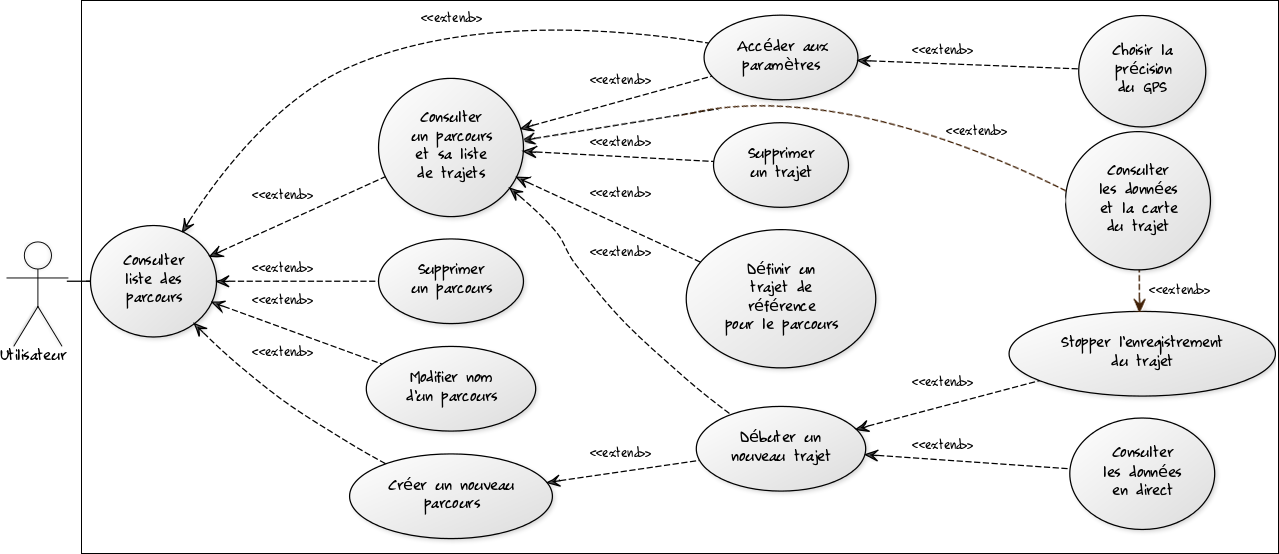
\includegraphics{img/DUC.png}
  \caption{Diagramme de cas d'utilisation de l'application}
\end{img}